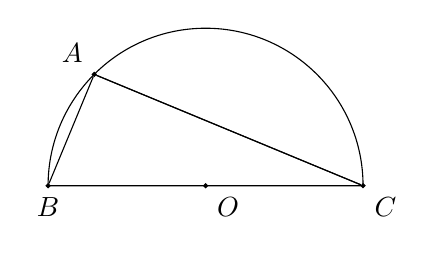
\begin{tikzpicture}
  [
    scale=2,
    >=stealth,
    point/.style = {draw, circle,  fill = black, inner sep = 0.5pt},
    dot/.style   = {draw, circle,  fill = black, inner sep = .2pt},
  ]

 \coordinate [point, label={below :	$B$ }] (B) at (-1, 0);
 \coordinate [point, label={below right:	$O$ }] (O) at (0, 0);
 \coordinate [point, label={below right:	$C$ }] (C) at (1, 0); 
 \coordinate [point, label={above left:	$A$ }] (A) at (-0.707,0.707);  
\draw (A) -- (C) arc(0:180:1) --cycle;
  \draw 
  (A) -- (B)
  (A) -- (C);
  \tkzMarkRightAngle[fill=blue!20,size=.2](B,A,C)    
%  \def\rad{1}

%  \draw (O) circle (\rad);  
%    \node (A) at +(45:{\rad}) [point,label = above right:$A$ $\brak{x,y}$] {};  
%  \path
%     (O)    edge  node[sloped, anchor=center, below, text width=0.5cm] { $r$}     (A) ; 
    
% \coordinate [point, label={below left:$B$}] (B) at (0, 0);
%    \node (A) at +(60:{2*sqrt(3)}) [label = above:$A$] {};
%  \coordinate [ label={below right:$C$ }] (C) at ($ (3,0) + sqrt(3)*(1,0) $);
%    \node (P) at +(30:{2*sqrt(3)}) [label = above:$P$] {};  
%  \path[->]
%     (B)    edge  node[sloped, anchor=center, below, text width=2.0cm] { $y = m_1x+c_1$}     (A) 
%	 (B)    edge  node[sloped, anchor=east, below, text width=2.0cm] { $y=m_2x+c_2$}     (C)
%	 (B)    edge  node[sloped, anchor=east, below, text width=2.0cm] { Bisector}     (P);
%  
%%  
%%  \coordinate [point, label={below left:$B$ $\brak{0,0}$}] (B) at (0, 0);
%%    \node (A) at +(60:{2*sqrt(3)}) [point, label = above:$A$ $\brak{a,b}$] {};
%%  \coordinate [point, label={below right:$C$ $\brak{c,0}$}] (C) at ($ (3,0) + sqrt(3)*(1,0) $);
%%  \node (D) at ({sqrt(3)},0) [point, label = below:$D$ $\brak{a,0}$] {};
%%    \node (E) at +(45:{(3+sqrt(3))/sqrt(2)}) [point, label = above right:$E$] {};
%%    \node (O) at +(45:{sqrt(6)}) [point, label = right:$O$] {};    
%%    \node (F) at +(60:{(3+sqrt(3))/2}) [point, label = left:$F$] {};        
%  \draw  (A) -- (B) -- (C);% -- (A);
%%  \node (D) at ($(B)!0.5!(C)$) [point, label = {below:$D$}]{};
%%  \draw (A) -- (D);  
%%  \draw (B) -- (E);    
%%  \draw[dashed] (C) -- (F);      
%\tkzMarkAngle[draw = black, fill = white, opacity=1](P,B,A)
%\tkzLabelAngle[pos = 0.8](P,B,A){$\theta$}
%\tkzMarkAngle[draw = black, fill = white, opacity=1,size=1.1](C,B,P)
%\tkzLabelAngle[pos = 0.9](C,B,P){$\theta$}

%\tkzMarkAngle[size=1.4,draw = black, fill = white, opacity=1](C,B,P)
%\tkzLabelAngle[pos=1.15,font=\scriptsize](C,B,P){$\theta$}

%  \tkzMarkAngle[fill=white,opacity=1,size=0.2,label={$\theta$},pos=0.2](P,B,A)  
%  \tkzMarkAngle[fill=blue!20,size=.4,label={$\theta$}](P,B,A)
%  \tkzMarkAngle[fill=blue!20,size=.2,label={$\theta$](C,B,P)
%  \tkzMarkRightAngle[fill=blue!20,size=.2](B,E,A)  
%  \path
%     (B)    edge  node[sloped, anchor=center, below, text width=2.0cm] { $k_1:1$}     (E)  
%	 (C)    edge  node[sloped, anchor=east, below, text width=2.0cm] { $1:k_2$}     (F);

\end{tikzpicture}

